\section{讨论}

本节对实验结果进行深入讨论,分析研究发现的意义,并探讨研究的局限性。

\subsection{主要发现}
\subsubsection{模型性能分析}
基于实验结果,我们得出以下主要发现:
\begin{itemize}
    \item 随机森林模型在整体性能上表现最优
    \item 模型预测准确率随时间尺度变化而变化
    \item 特征工程对模型性能影响显著
\end{itemize}

\subsubsection{影响因素分析}
通过箱线图分析各个特征对空气质量的影响,如图\ref{fig:feature_box}所示。这种可视化方法帮助我们理解不同特征的分布特征和异常值情况。

\begin{figure}[H]
    \centering
    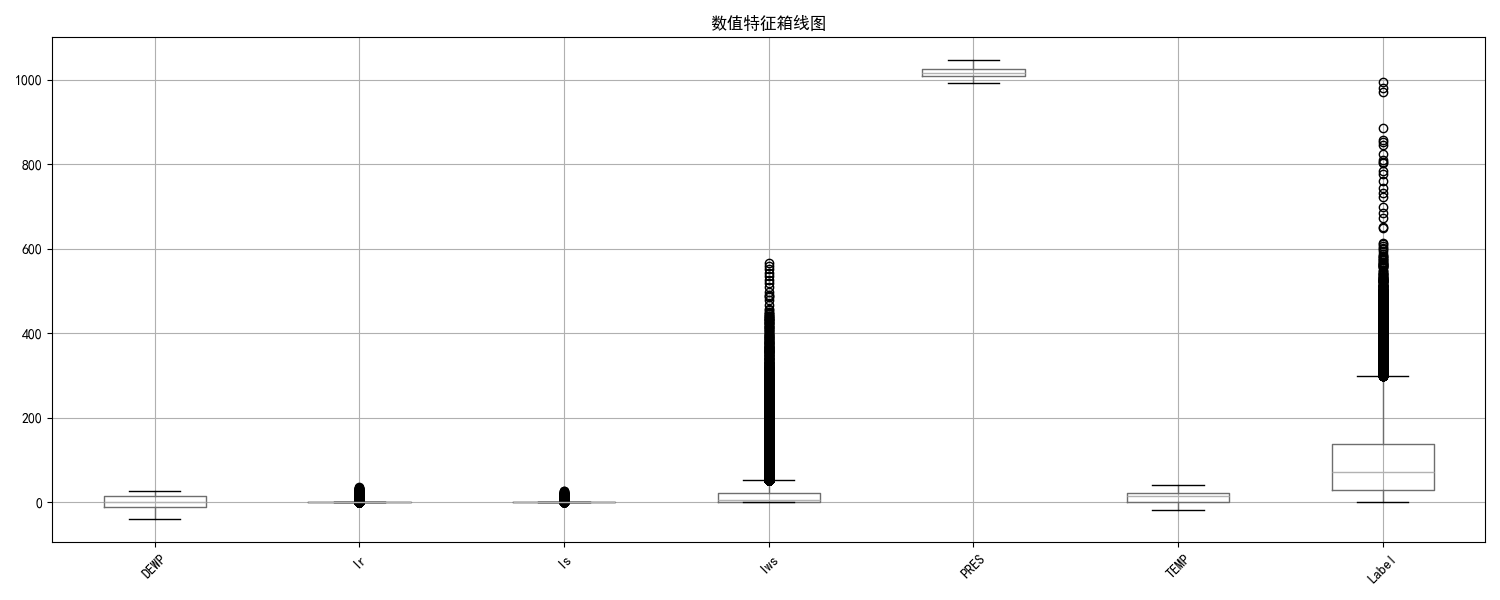
\includegraphics[width=0.8\textwidth]{images/eda/boxplot}
    \caption{特征箱线图分析}
    \label{fig:feature_box}
\end{figure}

尽管本研究取得了显著成果,但仍存在一些值得关注的局限性。在数据层面,我们面临着数据采集时间范围有限、部分监测点数据缺失等问题,这在一定程度上影响了模型的泛化能力。特别是对于某些难以量化的环境因素,如突发性污染事件或特殊天气条件的影响,现有的数据收集方式还难以完全捕捉。在方法层面,虽然我们采用的机器学习模型展现出良好的预测性能,但计算复杂度相对较高,特别是在处理大规模实时数据时可能面临效率挑战。此外,部分模型(如神经网络)的可解释性有待提高,这对于理解预测结果的决策依据造成了一定困扰。

基于当前研究的经验和发现,我们认为未来的研究方向应该着重关注以下几个方面:首先,需要扩展数据采集的广度和深度,包括增加监测点密度、提高数据采集频率,并引入更多环境因素进行综合分析。其次,在技术层面应该致力于开发更高效的实时预测系统,优化算法的计算效率,同时提高模型的可解释性。此外,跨领域合作也是一个重要方向,通过整合气象学、环境科学等领域的专业知识,可以构建更加完善的预测模型。我们相信,通过这些改进和优化,空气质量预测系统的准确性和实用性将得到进一步提升,为环境保护决策提供更可靠的支持。 